\renewcommand{\theequation}{\theenumi}
\renewcommand{\thefigure}{\theenumi}
\renewcommand{\thetable}{\theenumi}
\begin{enumerate}[label=\thesection.\arabic*.,ref=\thesection.\theenumi]
\numberwithin{equation}{enumi}
\numberwithin{figure}{enumi}
\numberwithin{table}{enumi}



\item Let $Y_1$ denote the first order statistic in a random sample of size $n$ from a distribution that has the pdf 
\begin{align}
    f(x) = 
    \begin{cases}
    e^{-(x-\theta)}&\text{ when } \theta<x<\infty\\
    0 &\text{  otherwise} 
    \end{cases}
\end{align}
Obtain the distribution of $Z_n = n(Y_1 - \theta)$.
%
\\
\solution
From the given information
\begin{align}
    Y_1 = \min\{X_1, X_2, ... X_n\}
\end{align}
%
and
\begin{align}
    F_{Z_n}(z) &= \pr{n(Y_1-\theta)\leq z}\\
    &= \pr{Y_1\leq \frac{z}{n} +\theta}\\
    &= 1-\pr{Y_1\ > \frac{z}{n} +\theta}\label{stats/1/eq_2}
\end{align}
%
Let
\begin{align}
    \brak{\dfrac{z}{n}+\theta} = z^{\prime}
\end{align}
%
Then
\begin{align}
    F_{Z_n}\brak{z}    &= 1-\prod_{i=1}^{n}\pr{X_i>z^{\prime}}\\
    &= 1-\brak{1-F(z^{\prime})}^n\\
    \implies F_{Z_n}(z) &= 1-\brak{1-F\brak{\frac{z}{n}+\theta}}^n\label{stats/1/eq_3}
\end{align}
%
where
%
\begin{align}
  F(x) &=\displaystyle\int\limits_{-\infty}^{x} f(t) \,dt\\
&=
    \begin{cases}
    1-e^{-(x-\theta)} &\text{when }\theta<x<\infty\\
    0 &\text{otherwise}
    \end{cases}
    \label{stats/1/eq_1}
\end{align}
%
Substituting from     \eqref{stats/1/eq_1} in \eqref{stats/1/eq_3},
\begin{align}
    F_{Z_n}(z) &=
    \begin{cases}
    1-e^{-n\brak{\frac{z}{n}+\theta-\theta}}&  \theta<\frac{z}{n}+\theta<\infty\\
    0&\text{otherwise}
    \end{cases}\\
    &= \begin{cases}
    1-e^{-z}&\text{when } 0<z<\infty\\
    0 &\text{otherwise}\label{stats/1/cdf}
    \end{cases}
\end{align}
and 
\begin{align}
    f_{Z_n}(z) &= \frac{d}{dz}F_{Z_n}(z)\\
    &=\begin{cases}
    e^{-z}& 0<z<\infty\\
    0&\text{otherwise}
    \end{cases}\label{stats/1/pdf}
\end{align}
The plots for the cdf in \eqref{stats/1/cdf} and the pdf in \eqref{stats/1/pdf} are shown in Fig. \ref{stats/1/fig_cdf} and Fig. \ref{stats/1/fig_pdf} respectively:
\begin{figure}[!ht]
    \centering
    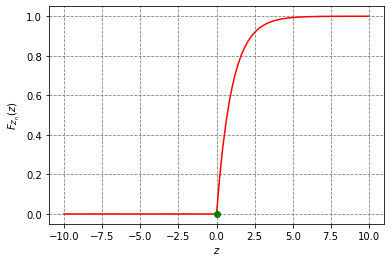
\includegraphics[width=\columnwidth]{stats/solutions/1/figures/cdf.png}
    \caption{cdf of $Z_n$}
    \label{stats/1/fig_cdf}
\end{figure}
\begin{figure}[!ht]
    \centering
    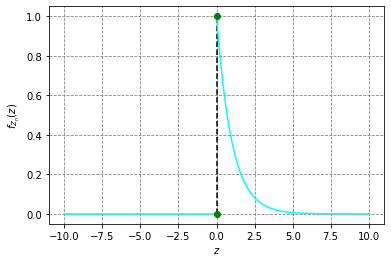
\includegraphics[width=\columnwidth]{stats/solutions/1/figures/pdf.png}
    \caption{pdf of $Z_n$}
    \label{stats/1/fig_pdf}
\end{figure}




%
\item Let $X_1, X_2, \ldots , X_n$ be a random sample of size $n \; ( \geq 2 ) $ from a distribution having the probability density function
\begin{align}
f(x;\theta) = 
\begin{cases}
\dfrac{1}{\theta} \exp\brak{-\dfrac{x}{\theta}} & x > 0, \\
0, & \text{otherwise,}
\end{cases}
\end{align}
where $\theta \in (0, \infty)$. Let $X_{(1)} = $ min $ \{ X_1, X_2, \ldots , X_n \} $ and $T = \sum_{i=1}^n X_i $. Then $E(X_{(1)} | T)$ equals 
\begin{enumerate}[label = (\Alph*)]
\item $\dfrac{T}{n^2}$ \\
\item $\dfrac{T}{n}$ \\
\item $\dfrac{(n+1)T}{2n}$ \\
\item $\dfrac{(n+1)^2 T}{4n^2}$
\end{enumerate}
\solution
\begin{lemma}
    {\em Lehmann–Scheffé theorem :} If $T$ is a complete sufficient statistic for $\theta$ and 
    \begin{align}
    \label{stats/2/eqn 2.0.1}
    E(g(T)) = \tau(\theta)
    \end{align}
    then $g(T)$ is the uniformly minimum-variance unbiased estimator (UMVUE) of $\tau(\theta)$.
    
\end{lemma}




We know that 
\begin{align}
T = \sum_{i=1}^{n} X_i
\end{align}
is a complete and sufficient statistic. By the law of total expectation, 
\begin{align}
\label{stats/2/eqn 2.0.3}
E\brak{E(X_{(1)} | T )} = E(X_{(1)})
\end{align}
By Lehmann–Scheffé theorem, with
\begin{align}
\theta &= X_{(1)},\\ 
\tau(x) &= E(x),\\
g(T) &= E(X_{(1)} | T).
\end{align}
it follows from \eqref{stats/2/eqn 2.0.3} that $E(X_{(1)} | T)$ is the UMVUE of $E(X_{(1)})$.
\begin{align}
\pr{X_{(1)} > x} &= \pr{X_1 > x}\ldots \pr{X_n > x}\\
&= (1-F_{X_{1}}(x))\ldots(1-F_{X_{n}}(x))\\
&= (1-F_{X_{1}}(x))^n \\
&= \exp\brak{-\frac{nx}{\theta}}\\
F_{X_{(1)}}(x) &= 1 - \exp\brak{-\frac{nx}{\theta}}\\
f_{X_{(1)}}(x) &= \frac{n}{\theta} \exp\brak{-\frac{nx}{\theta}}
\end{align}
Therefore, $X_{(1)}$ follows an exponential distribution with mean $\dfrac{\theta}{n}$.
\begin{align}
E(X_{(1)}) = \frac{\theta}{n}
\end{align}
Note that,
\begin{align}
E\brak{\frac{T}{n^2}} &= E\brak{\frac{\sum_{i=1}^n X_i}{n^2}}\\
&= \frac{E(\sum_{i=1}^n X_i)}{n^2}\\
&= \sum_{i=1}^n \frac{E(X_i)}{n^2}\\
&= \sum_{i=1}^n \frac{\theta}{n^2}\\
&= \frac{\theta}{n}\\
&= E(X_{(1)})
\end{align}
Therefore, by Lehmann–Scheffé theorem, with
\begin{align}
\theta &= X_{(1)},\\
\tau(x) &= E(x),\\
g(T) &= \frac{T}{n^2},
\end{align}
it follows that $\dfrac{T}{n^2}$ is UMVUE of $E(X_{(1)})$.\\

Since there exists a unique UMVUE for $E(X_{(1)})$, it follows that 
\begin{align}
E(X_{(1)} | T) = \frac{T}{n^2}
\end{align}
Hence, option A is correct.
\begin{figure}[!hbt]
    \centering
	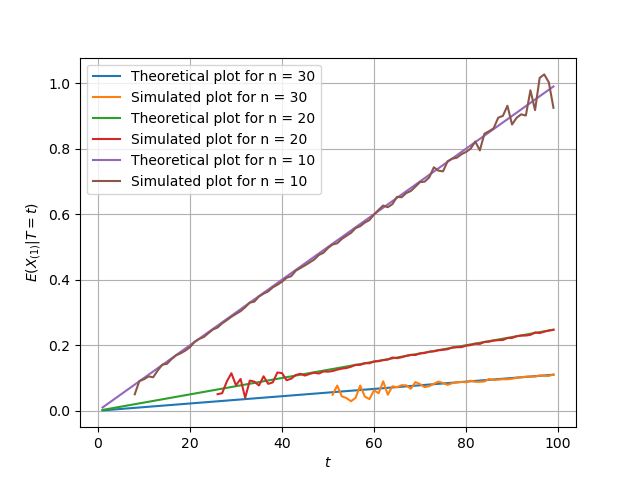
\includegraphics[width=\columnwidth]{stats/solutions/2/Figures/Figure_1.png}
    \caption{Theory vs Simulated plot of $E(X_{(1)} |T)$}
    \label{stats/2/CDF_Y}
\end{figure}

%
\item Suppose n units are drawn from a population of N units sequentially as follows. A random sample
\begin{align}
    U_1, U_2, ... U_N \text{ of size N, drawn from }U\brak{0, 1} 
\end{align} 
The k-th population unit is selected if 
\begin{align}
    U_k<\frac{n - n_k}{N-k+1}, k = 1, 2, ..N. \text{where, } n_1=0, n_k = 
\end{align}
number of units selected out of first k-1 units for each k = 2, 3, ..N. Then,
\begin{enumerate}
    \item The probability of inclusion of the second unit in the sample
    \begin{align}
        \text{ is } \frac{n}{N}
    \end{align}
    \item The probability of inclusion of the first and the second unit in the sample
    \begin{align}
        \text{ is } \frac{n \brak{n-1}}{N \brak{N-1}}
    \end{align}
    \item The probability of not including the first and including the second unit in the sample
    \begin{align}
        \text{ is } \frac{n \brak{N-n}}{N \brak{N-1}}
    \end{align}
    \item The probability of including the first and not including the second unit in the sample
    \begin{align}
        \text{ is } \frac{n \brak{n-1}}{N \brak{N-1}}
    \end{align}
\end{enumerate}
%
\solution
\input{solutions/2018/dec/116.tex}
%
%
\item Let $X_{1},X_{2},X_{3},..,X_{n}$ be independent random variables follow a common continuous distribution \textbf{F}, which is symmetric about 0. For i=1,2,3,..n, define 
\begin{align}
\tag{1.1}
\label{eq1}
S_{i} = 
\begin{cases}
1 & if \hspace{0.2cm}X_{i}>0
\\
-1 & if\hspace{0.2cm} X_{i}<0 \hspace{0.2cm} and
\\
0 & if \hspace{0.2cm}X_{i}=0
\end{cases}
\end{align}
$R_{i}$=rank of $|X_{i}|$ in the set\{$|X_{1}|,|X_{2}|,..,|X_{n}|$\}.Which of the following statements are correct?
\begin{enumerate}
\item $S_{1},S_{2},..,S_{n}$ are independent and identically distributed.
\item $R_{1},R_{2},..,R_{n}$ are independent and identically distributed.
\item $S=\brak{S_{1},S_{2},..,S_{n}}$ and $R=\brak{ R_{1},R_{2},..,R_{n}}$ are independent.
\end{enumerate}
%
\solution

A sequence $\{X_{i}\}$ is an Independent and identical if and only if 
$F_{X_{n}}(x)=F_{X_{k}}(x)$
$\forall$ n,k,x and any subset of terms of the sequence is a set of mutually independent random variables.
Where F is the probability density function.
\begin{enumerate}
\item As the probability distribution function of $\{X_{i}\}$ is symmetric about origin we can say that 
\begin{equation}
\tag{2.1}
  F_{X_{i}}(-x)=F_{X_{i}}(x)    \forall x \in R  
\end{equation}
and the mean of the distribution($\mu$)
\begin{equation}
    \tag{2.2}
    \mu=0
\end{equation}
The sequence $S_{i}$ depend on $X_{i}$ as mention in \ref{eq1}, as each $S_{i}$ depend only on $X_{i}$ we can say that sequence $S_{i}$ is independent.
\begin{equation}
    \tag{2.3}
\pr{S_{1}=1,S_{2}=1,...,S_{n}=1}=\Pi_{i=1}^{n}\pr{S_{i}=1}
\end{equation}
Any subset of terms of sequence $\{S_{i}\}$ is a set of mutually independent random variables and its distribution is identical. 
\begin{align}
    \tag{2.4}
    F_{S_{n}}(s)=F_{S_{k}}(s) \hspace{0.5cm} \forall s,k,n
\end{align}
So, the sequence $\{S_{i}\}$ is independent and identical.
\item 
\textbf{Ranking} refers to the data transformation in which the numerical or ordinary values are replaced by the rank of numerical value when compared to a list of other values.Usually we follow increasing order for ranking.\\
Ranking of a sequence depend on every elements of the sequence.Let $\{R_{i}\}$ be the output sequence of the ranking function of $\{|X_{i}|\}$.
\begin{equation}
    \tag{2.5}
    R_{k}=\text{rank of $|X_{k}|$ in the set\{$|X_{1}|,|X_{2}|,..,|X_{n}|$\}}
\end{equation}
As $R_{k}$ depend not only on $|X_{k}|$ but on the rest of the elements of the set\{$|X_{1}|,|X_{2}|,..,|X_{n}|$\}. So the sequence $R_{i}$ is not independent. Hence $R_{i}$ is not an independent and identical distribution.
\item 
As the $i^{th}$ element of sequence R depends only on set\{$|X_{1}|,|X_{2}|,..,|X_{n}|$\}, we can say that sequence S and R are independent.
\end{enumerate}
Answer:A,C
%
%
\item A simple random variable of size n will be drawn from a class of 125 students, and the mean mathematics score of the sample will be computed, If the standard error of the sample mean for "with replacement sampling" is twice as much as the standard error of the sample mean for "without replacement sampling", the value of n is ? 
	\begin{enumerate}
	\item 32
	\item 63
	\item 79
	\item 94
	\end{enumerate}
%
\solution
Let N be the population size so, N=120. The given sample size is n.
\textbf{Notations :}
y : student under consideration.
$y_i$ : Maths marks of $i^{th}$ student in the sample.
Y : student of class.
$Y_i$ : Maths marks of $i^{th}$ student in the class.
$\overline{y}=\dfrac{1}{n}\sum_{i=1}^{n}y_i$ : Average of sample class.
$\overline{Y}=\dfrac{1}{N}\sum_{i=1}^{N}Y_i$ : Average of whole class.
$S^2 = \dfrac{1}{N-1} \sum_{i=1}^{N} (Y_i-\bar{Y})^2$ : S=Std dev of the class.
$\sigma^2=\dfrac{1}{N} \sum_{i=1}^{N} (Y_i-\bar{Y})^2$ : Variance of the class.
Standard error of sample mean $SE_{mean}=\dfrac{s}{\sqrt{n}}$.\\
Where 
\begin{align*}
s & = \text{standard deviation of sample mean.}\\
n & = \text{sample class size.}
\end{align*}
\textbf{Variance of the $\overline{y}$}
\begin{align}
& V(\overline{y})= E(\overline{y}-\overline{Y})^2\\
& = E\left[\dfrac{1}{n} \sum_{i=1}^{n}(y_i-\overline{Y})\right]^2\\
& = E\left[\dfrac{1}{n^2} \sum_{i=1}^{n} (y_i-\overline{Y})^2 + \dfrac{1}{n^2} \underset{1\leq i\neq j\leq n}{\sum\sum}\, (y_i-\overline{Y})(y_j-\overline{Y})\right]\\
& = \dfrac{1}{n^2}\sum_{i=1}^{n} E(y_i-\overline{Y})^2+\dfrac{1}{n^2} \underset{1\leq i\neq j\leq n}{\sum\sum}\, E(y_i-\overline{Y})(y_j-\overline{Y})\\
& \text{Let } K=\underset{1\leq i\neq j\leq n}{\sum\sum}\, E(y_i-\overline{Y})(y_j-\overline{Y})\\
& = \dfrac{1}{n^2}\sum_{i=1}^{n} \sigma^2 + \dfrac{K}{n^2}\\
& = \dfrac{1}{n^2} n \sigma^2 +\dfrac{K}{n^2}\\
& = \dfrac{N-1}{Nn} S^2+\dfrac{K}{n^2}\label{june2018-58:eq_1}
\end{align}
Finding the value of K in case of Simple random sampling with repetition (SRSWR)and Simple random sampling without repetition(SRSWOR) allows us to calculate the variance of mean.
\vspace{0.5 cm}
\textbf{K value in case of SRSWOR}
\begin{align*}
&K=\underset{1\leq i\neq j\leq n}{\sum\sum}\, E(y_i-\overline{Y})(y_j-\overline{Y})
\end{align*}
Consider
\begin{multline*}
E(y_i-\overline{Y})(y_j-\overline{Y})= \\
\dfrac{1}{N(N-1)}\underset{1\leq k\neq l\leq n}{\sum\sum}\, E(y_k-\overline{Y})(y_l-\overline{Y})
\end{multline*}
Since
\begin{multline*}
\left[\sum_{k=1}^N(y_k-\overline{Y})\right]^2=\sum_{i=1}^{N}(y_k-\overline{Y})^2+\\
\underset{1\leq k\neq l\leq n}{\sum\sum}\, E(y_k-\overline{Y})(y_l-\overline{Y})
\end{multline*}
\begin{align*}
&\implies 0 = (N-1)S^2+\underset{1\leq k\neq l\leq n}{\sum\sum}\, E(y_k-\overline{Y})(y_l-\overline{Y})\\
& \implies E(y_i-\overline{Y})(y_j-\overline{Y})=\dfrac{1}{N(N-1)}(N-1)(-S^2)\\
& \implies K = n(n-1)\dfrac{(-S^2)}{N}
\end{align*}
Putting this value in (\ref{june2018-58:eq_1}) gives us 
\begin{align}
V(\overline{y})_{WOR} & = \dfrac{N-1}{Nn} S^2+ \dfrac{n-1(-S^2)}{Nn}\\
& = \dfrac{N-n}{Nn} S^2 \label{june2018-58:eq_2}
\end{align}
\textbf{K value in case of SRSWR}
\begin{align*}
&K=\underset{1\leq i\neq j\leq n}{\sum\sum}\, E(y_i-\overline{Y})(y_j-\overline{Y})
\end{align*}
Since we are selecting the samples with replacements choosing $i^{th}$ and $j^{th}$ sample is independent of each other. So,
\begin{align*}
K&=\underset{1\leq i\neq j\leq n}{\sum\sum}\, E(y_i-\overline{Y})E(y_j-\overline{Y})\\
& = 0\\
& \text{(Since deviation about mean is 0)}
\end{align*}
Putting K=0 in (\ref{june2018-58:eq_1}) we get 
\begin{align}
V(\overline{y})_{WR} & = \dfrac{N-1}{Nn} S^2\label{june2018-58:eq_3}
\end{align}
From equation \eqref{june2018-58:eq_2}  standard error of mean of sample class without repetition
\begin{align}
{SE}_{WOR} & = \dfrac{s}{\sqrt{n}}\\
& = \sqrt{\dfrac{V(\overline{y})_{WOR}}{n}}\\
& = \sqrt{\dfrac{N-n}{Nn^2}}S \label{june2018-58:eq_4}
\end{align} 
From equation \eqref{june2018-58:eq_3}  standard error of mean of sample class with repetition
\begin{align}
{SE}_{WR} & = \sqrt{\dfrac{V(\overline{y})_WR}{n}}\\
& = \sqrt{\dfrac{N-1}{Nn^2}}S \label{june2018-58:eq_5}
\end{align}
Given to find the value of n if $2 \times {SE}_{WOR} =  {SE}_{WR}$.
From \eqref{june2018-58:eq_4} and \eqref{june2018-58:eq_5} we can write 
\begin{align}
& 2\sqrt{\dfrac{N-n}{Nn^2}}S= \sqrt{\dfrac{N-1}{Nn^2}}S\\
\implies & 4(N-n) = N-1\\
\implies & 4N+1-N=4n\\
\implies & 4n=3(125)+1\\
\implies & n=94
\end{align}
Therefore the sample size for the given condition to be met is n=94.(\textbf{Option D})


%
\item Let $X_1$ and $X_2$ be i.i.d. with probability mass function $f_{\theta}\brak{x} = \theta^x \brak{1-\theta}^{1-x}$; $x=0,1$ where $\theta \in \brak{0,1}$. Which of the following statements are true?
\begin{enumerate}
    \item $X_1 + 2X_2 $ is a sufficient statistic
    \item $X_1 - X_2 $ is a sufficient statistic
    \item $X_1^2 + X_2^2 $ is a sufficient statistic
    \item $X_1^2 + X_2 $ is a sufficient statistic
\end{enumerate}
%
\solution
Given that, $X_1$ and $X_2$ are i.i.d. with probability mass function
\begin{align}
    f\brak{x} = 
    \begin{cases}
    \brak{1-\theta} & x=0\\
    \theta & x=1
    \end{cases}
\end{align}
A statistic $t=T\brak{X}$ is sufficient for a parameter $\theta$ if the conditional probability distribution of the data, given the statistic $t=T\brak{X}$ does not depend on the parameter $\theta$. i.e,
\begin{align}
    P_\theta\brak{X_1=x_1,X_2=x_2|T=t}
\end{align}
is independent of $\theta$ for all $x_1,x_2$ and $t$
\begin{enumerate}
    \item Let $T=X_1+2X_2$\\
    Consider a case where $x_1=0, x_2=0$ and $t=0$
    \begin{align}
    \pr{T=0}&=\pr{X_1+2X_2=0}\\
    \label{june2018-108:eq1}&=\pr{X_1=0,X_2=0}
    \end{align}
    As $X_1$ and $X_2$ are independent
    \begin{multline}
        \pr{T=0}=\pr{X_1=0}\pr{X_2=0}\\
        =\brak{1-\theta}^2
    \end{multline}
   The conditional probability,
    \begin{multline}
        \pr{X_1=0,X_2=0 | T=0}\\
        =\frac{\pr{\brak{X_1=0,X_2=0}\cap\brak{T=0}}}{\pr{T=0}}
    \end{multline}
    From \eqref{june2018-108:eq1}, $\brak{X_1=0,X_2=0} \subseteq \brak{T=0}$
    \begin{multline}
        =\frac{\pr{X_1=0,X_2=0}}{\pr{T=0}}=\frac{\brak{1-\theta}^2}{\brak{1-\theta}^2}=1
    \end{multline}
    Similarly, conditional probabilities for other values of $x_1,x_2$ and $t$ are given in table \ref{june2018-108:table1}
    \begin{table}[h!]
    \begin{tabular}[width=\columnwidth]{|c|c|c|c|}
         \hline
        \multirow{2}{*}{$x_1$} & \multirow{2}{*}{$x_2$} & t & Conditional probability\\
        & & $t=X_1+2X_2$ & $P_\theta\brak{X_1=x_1,X_2=x_2|T=t}$\\
        \hline
        \multirow{2}{*}{0} & \multirow{2}{*}{0} & 0 & 1\\ 
        & & otherwise & 0 \\ 
        \hline
        \multirow{2}{*}{1} & \multirow{2}{*}{0} & 1 & 1\\ 
        & & otherwise & 0 \\ 
        \hline
        \multirow{2}{*}{0} & \multirow{2}{*}{1} & 2 & 1\\ 
        & & otherwise & 0 \\ 
        \hline
        \multirow{2}{*}{1} & \multirow{2}{*}{1} & 3 & 1\\ 
        & & otherwise & 0 \\        
        \hline
    \end{tabular}
    \caption{Conditional Probabilities}
    \label{june2018-108:table1}
    \end{table}    
    
    From table \ref{june2018-108:table1}, all the conditional probabilities are independent of $\theta$\\ $\therefore X_1+2X_2$ is a sufficient statistic.
    
    
    \item Let $T=X_1-X_2$\\
    Consider a case where $x_1=0, x_2=0$ and $t=0$
    \begin{multline}
        \label{june2018-108:eq2}\pr{T=0}=\pr{X_1-X_2=0}\\=\pr{X_1=0,X_2=0}+\pr{X_1=1,X_2=1}
    \end{multline}
    As $X_1$ and $X_2$ are independent
    \begin{multline}
        =\pr{X_1=0}\pr{X_2=0}\\+\pr{X_1=1}\pr{X_2=1}=\brak{1-\theta}^2 + \theta^2
    \end{multline}
    The conditional probability,
    \begin{multline}
        \pr{X_1=0,X_2=0 | T=0}\\
        =\frac{\pr{\brak{X_1=0,X_2=0}\cap\brak{T=0}}}{\pr{T=0}}
    \end{multline}
    From \eqref{june2018-108:eq2}, $\brak{X_1=0,X_2=0} \subseteq \brak{T=0}$
    \begin{multline}
        =\frac{\pr{X_1=0,X_2=0}}{\pr{T=0}}=\frac{\brak{1-\theta}^2}{\brak{1-\theta}^2 + \theta^2}
    \end{multline}
  
    depends on $\theta$. \\
    $\therefore X_1-X_2$ is not a sufficient statistic.
    
    \item Let $T=X_1^2+X_2^2$\\
    Consider a case where $x_1=1, x_2=0$ and $t=1$
    \begin{multline}
        \label{june2018-108:eq3}\pr{T=1}=\pr{X_1^2+X_2^2=1}\\=\pr{X_1=1,X_2=0}+\pr{X_1=0,X_2=1}\\=\theta \brak{1-\theta} + \brak{1-\theta}\theta  = 2\theta \brak{1-\theta}
    \end{multline}
    The conditional probability,
    \begin{multline}
        \pr{X_1=1,X_2=0 | T=1}\\
        =\frac{\pr{\brak{X_1=1,X_2=0}\cap\brak{T=0}}}{\pr{T=1}}
    \end{multline}
    From \eqref{june2018-108:eq3}, $\brak{X_1=1,X_2=0} \subseteq \brak{T=1}$
    \begin{multline}
        =\frac{\pr{X_1=1,X_2=0}}{\pr{T=1}}=\frac{\theta\brak{1-\theta}}{2\theta\brak{1-\theta}}=\frac{1}{2}
    \end{multline}
    Similarly, conditional probabilities for other values of $x_1,x_2$ and $t$ are given in table \ref{june2018-108:table2}
    \begin{table}[h!]
    \begin{tabular}[width=\columnwidth]{|c|c|c|c|}
         \hline
        \multirow{2}{*}{$x_1$} & \multirow{2}{*}{$x_2$} & t & Conditional probability\\
        & & $t=X_1^2+X_2^2$ & $P_\theta\brak{X_1=x_1,X_2=x_2|T=t}$\\
        \hline
        \multirow{2}{*}{0} & \multirow{2}{*}{0} & 0 & 1\\ 
        & & otherwise & 0 \\ 
        \hline
        \multirow{2}{*}{1} & \multirow{2}{*}{0} & 1 & $\frac{1}{2}$\\ 
        & & otherwise & 0 \\ 
        \hline
        \multirow{2}{*}{0} & \multirow{2}{*}{1} & 1 & $\frac{1}{2}$\\ 
        & & otherwise & 0 \\ 
        \hline
        \multirow{2}{*}{1} & \multirow{2}{*}{1} & 2 & 1\\ 
        & & otherwise & 0 \\        
        \hline
    \end{tabular}
    \caption{Conditional Probabilities}
    \label{june2018-108:table2}
    \end{table}  
    
    From table \ref{june2018-108:table2}, all the conditional probabilities are independent of $\theta$\\ $\therefore X_1^2+X_2^2$ is a sufficient statistic.
    
    \item Let $T=X_1^2+X_2$\\
    Consider a case where $x_1=1, x_2=0$ and $t=1$
    \begin{multline}
        \label{june2018-108:eq4}\pr{T=1}=\pr{X_1^2+X_2=1}\\=\pr{X_1=1,X_2=0}+\pr{X_1=0,X_2=1}\\=\theta \brak{1-\theta} + \brak{1-\theta}\theta  = 2\theta \brak{1-\theta}
    \end{multline}
    The conditional probability,
    \begin{multline}
        \pr{X_1=1,X_2=0 | T=1}\\
        =\frac{\pr{\brak{X_1=1,X_2=0}\cap\brak{T=0}}}{\pr{T=1}}
    \end{multline}
    From \eqref{june2018-108:eq4}, $\brak{X_1=1,X_2=0} \subseteq \brak{T=1}$
    \begin{multline}
       =\frac{\pr{X_1=1,X_2=0}}{\pr{T=1}}=\frac{\theta\brak{1-\theta}}{2\theta\brak{1-\theta}}=\frac{1}{2}
    \end{multline}
    Similarly, conditional probabilities for other values of $x_1,x_2$ and $t$ are given in table \ref{june2018-108:table3}
    
    \begin{center}
    \begin{table}[h!]
    \begin{tabular}[width=\columnwidth]{|c|c|c|c|}
         \hline
        \multirow{2}{*}{$x_1$} & \multirow{2}{*}{$x_2$} & t & Conditional probability\\
        & & $t=X_1^2+X_2$ & $P_\theta\brak{X_1=x_1,X_2=x_2|T=t}$\\
        \hline
        \multirow{2}{*}{0} & \multirow{2}{*}{0} & 0 & 1\\ 
        & & otherwise & 0 \\ 
        \hline
        \multirow{2}{*}{1} & \multirow{2}{*}{0} & 1 & $\frac{1}{2}$\\ 
        & & otherwise & 0 \\ 
        \hline
        \multirow{2}{*}{0} & \multirow{2}{*}{1} & 1 & $\frac{1}{2}$\\ 
        & & otherwise & 0 \\ 
        \hline
        \multirow{2}{*}{1} & \multirow{2}{*}{1} & 2 & 1\\ 
        & & otherwise & 0 \\        
        \hline
    \end{tabular}
    \caption{Conditional Probabilities}
    \label{june2018-108:table3}
    \end{table}  
    \end{center}
    From table \ref{june2018-108:table3}, all the conditional probabilities are independent of $\theta$\\
    $\therefore X_1^2+X_2$ is a sufficient statistic.
    
\end{enumerate}
\rightline{Answer : Options 1,3,4}

%
%
\item Let X$_{1}$ and X$_{2}$ be a random sample of size two
from a distribution with probability density
function
\begin{align}
    f_{\theta}(x) &= \theta \brak{\dfrac{1}{\sqrt{2\pi}}}e^{-\dfrac{1}{2} x^{2}} + \brak{1-\theta}\brak{\dfrac{1}{2}}e^{-\mid x\mid} \nonumber,
\end{align}
$-\infty<x<\infty$,\\
where  $\theta \in \cbrak{ 0,\dfrac{1}{2}, 1 }$. If the observed values
of X$_{1}$ and X$_{2}$ are 0 and 2, respectively, then
the maximum likelihood estimate of $\theta$ is
\begin{enumerate}
    \item 0 
    \item $\frac{1}{2}$
    \item 1
    \item not unique
\end{enumerate}
%
\solution
Given X$_{1}=$0, X$_{2}=$2, n=2 and
\begin{align}
    f_{\theta}(x) =\theta \brak{\dfrac{1}{\sqrt{2\pi}}}e^{-\dfrac{1}{2} x^{2}} + \brak{1-\theta}\brak{\dfrac{1}{2}}e^{-\mid x\mid}
\end{align}
Then log of likelihood function is given by
\begin{align}
l(\theta) &= \sum_{i=1}^{i=n} \log f_{\theta}(x_{i})\\
&= \log f_{\theta}(x_{1}) + \log f_{\theta}(x_{2}) \\
&=\log\brak{\theta\brak{\dfrac{1}{\sqrt{2\pi}}}e^{-\dfrac{1}{2}0^{2}}+\brak{1-\theta}\brak{\dfrac{1}{2}}e^{-\mid 0\mid}} \nonumber\\&\hspace{0.75cm}+\log\brak{\theta\brak{\dfrac{1}{\sqrt{2\pi}}} e^{-\dfrac{1}{2}2^{2}}+\brak{1-\theta}\brak{\dfrac{1}{2}}e^{-\mid 2\mid}}
\end{align}
\begin{align}
&=\log\brak{\theta\brak{\dfrac{1}{\sqrt{2\pi}}}+(1-\theta)\brak{\dfrac{1}{2}}}\nonumber\\&\hspace{0.75cm}+\log\brak{\theta\brak{\dfrac{1}{\sqrt{2\pi}}} e^{-2}+\brak{1-\theta}\brak{\dfrac{1}{2}}e^{-2}}\\
&=2\log\brak{\theta\brak{\dfrac{1}{\sqrt{2\pi}}}+\brak{1-\theta}\brak{\dfrac{1}{2}}} -2
\end{align}
Since likelihood $L(\theta) = e^{l(\theta)}$.\\ \\
Likelihood function $L(\theta)$  at $\theta = 0, \frac{1}{2}, 1$ is given by
\begin{enumerate}
    \item At $\theta=0$ \hspace{0.5cm} $L(\theta=0)=\frac{1}{4}e^{-2}=0.0338$\\
    \item At $\theta=1$ \hspace{0.5cm} $L(\theta=1)=\frac{1}{2\pi}e^{-2}=0.0215$\\
    \item At $\theta=\frac{1}{2}$ \hspace{0.2cm}
    $L(\theta=\frac{1}{2})=\brak{\frac{1}{2\sqrt{2\pi}}+\frac{1}{4}}^{2}e^{-2}=0.0273$
\end{enumerate}
Hence the maximum likelihood estimate of $\theta$ is at $\theta=0$

%
%
\item Let $\left\{X_{n}, n \geq 1\right\}$ be i.i.d. uniform (-1,2) random variables. Which of the following statements are true?
\begin{enumerate}[label=\alph*)]
\item $\dfrac{1}{n} \sum_{i=1}^{n} X_{i} \rightarrow 0$ almost surely
\item $\left\{\dfrac{1}{2 n} \sum_{i=1}^{n} X_{2 i}-\dfrac{1}{2 n} \sum_{i=1}^{n} X_{2 i-1}\right\}\rightarrow 0$
almost surely
\item $\sup \left\{X_{1}, X_{2}, \ldots\right\}=2$ almost surely
\item $\inf \left\{X_{1}, X_{2}, \ldots\right\}=-1$ almost surely
\end{enumerate}
\solution
We using convergence in almost surely and Strong law of large number (SLLN)
\begin{enumerate}
\item {\em Almost sure convergence : }Let $X_{1}, X_{2}, \ldots$ be an infinite sequence of random variables. We shall say that the sequence $\left\{X_{i}\right\}$ converges with probability 1 (or converges almost surely (a.s.)) to a random variable $Y$, if 
\begin{align}
\pr{\lim _{n \rightarrow \infty} X_{n}=Y}=1 \\ 
\text{and we write}, X_{n} \stackrel{a . s .}{\rightarrow} Y
\end{align} 
\item {\em SLLN : }Let $X_{n}$ be i.i.d with $\mathbf{E}\left[\left|X_{1}\right|\right]<\infty$. Then, as $n \rightarrow \infty$ , we have
\begin{align}
\dfrac{S_{n}}{n} \stackrel{\text { a.s. }}{\rightarrow} \mathbf{E}\left[X_{1}\right]\implies \dfrac{S_{n}}{n} \stackrel{\text { P }}{\rightarrow} \mathbf{E}\left[X_{1}\right]\\
,\text{where} \, S_n = X_1 + \cdots + X_n
\end{align}   
also,
\begin{align}
X_i \stackrel{a.s.}{\rightarrow} X \implies g(X_i) \stackrel{a.s.}{\rightarrow} g(X)
\label{june/2017/104Eq}  
\end{align}
\end{enumerate}
\begin{enumerate}[label=\alph*)]
\item\begin{align}
\dfrac{1}{n}\left(X_{1}+\cdots+X_{n}\right) \rightarrow E(X)\in(-1,2)\\
\text{as} \, n\rightarrow\infty,
\end{align}
according to strong law of large numbers (SLLN).\\
So, option $(\mathrm{A})$ is incorrect.
\item using this \ref{june/2017/104Eq} , we solve as
\begin{align}
\left\{\dfrac{1}{2 n} \sum_{i=1}^{n} X_{2 i}-\dfrac{1}{2 n} \sum_{i=1}^{n} X_{2 i-1}\right\}&\stackrel{a.s.}{\rightarrow}\left\{\dfrac{nX}{2 n}-\dfrac{nX}{2 n}\right\}\\
&=0
\end{align}
option $(\mathrm{B})$ is correct.
\item  Similarly, Let $M=\sup (S) .$ Then,
\begin{align}
x \leq M, &\quad \forall x \in S \\
\forall \epsilon>0,& \quad(M-\epsilon, M] \cap S \neq \emptyset
\end{align}
where, $S$ be a nonempty subset of $\mathbb{R}$ with an upper bound. Using $X_i \stackrel{a.s.}{\rightarrow} X$ this , we  conclude that
\begin{align}
\sup \left\{X_{1}, X_{2}, \ldots\right\}&=2 \;almost\; surely
\end{align}
\item Let $m=\inf (S)$. Then
\begin{align}
x \geq m, & \quad \forall x \in S \\
\forall \epsilon>0, &\quad {[m, m+\epsilon] \cap S \neq \emptyset}
\end{align}
where, $S$ be a nonempty subset of $\mathbb{R}$ with an lower bound. Again using $X_i \stackrel{a.s.}{\rightarrow} X$ this , we conclude that
\begin{align}
\inf \left\{X_{1}, X_{2}, \ldots\right\}&=-1 \;almost\; surely
\end{align}
Hence $(\mathrm{B}),(\mathrm{C})$ and $(\mathrm{D})$ are correct options.
\end{enumerate}
%
\item $X_{1}, X_{2}, \cdots$ are independent identically distributed random variables
having common density $f$. Assume $f(x)=f(-x)$ for all $x \in \mathbb{R}$. Which of the following statements is correct?
\begin{enumerate}[label=\alph*)]
\item $\dfrac{1}{n}\left(X_{1}+\cdots+X_{n}\right) \rightarrow 0$ in probability
\item $\dfrac{1}{n}\left(X_{1}+\cdots+X_{n}\right) \rightarrow 0$ almost surely
\item $\pr{\dfrac{1}{\sqrt{n}}\left(X_{1}+\cdots+X_{n}\right)<0} \rightarrow \dfrac{1}{2}$
\item $\sum_{i=1}^{n} X_{i}$ has the same distribution as $\sum_{i=1}^{n}(-1)^{i} X_{i}$
\end{enumerate}
%
\solution
We using
\begin{enumerate}[label=\alph*)]
\item 
\begin{enumerate}[label=(\arabic*)]
\item {\em Convergence in probability : }Let $X_{1}, X_{2}, \ldots$ be an infinite sequence of random variables, and let $Y$ be another random variable. Then the sequence $\left\{X_{n}\right\}$ converges in probability to $Y$, if
\begin{align}
\forall \epsilon>0, \lim _{n \rightarrow \infty} \pr{\left|X_{n}-Y\right| \geq \epsilon}=0,
\end{align}
and we write 
\begin{align}
X_{n} \stackrel{P}{\rightarrow} Y.
\end{align}
\item {\em Convergence in almost surely : }Let $X_{1}, X_{2}, \ldots$ be an infinite sequence of random variables. We shall say that the sequence $\left\{X_{i}\right\}$ converges with probability 1 (or converges almost surely (a.s.)) to a random variable $Y$, if 
\begin{align}
\pr{\lim _{n \rightarrow \infty} X_{n}=Y}=1
\end{align}
and we write
\begin{align}
X_{n} \stackrel{a . s .}{\rightarrow} Y
\end{align}
\item {\em Strong law of large number(SLLN) : }Let $X_{1}, X_{2}, \ldots$ be an infinite sequence of random variables, If $\mathbf{E}\left[\left|X_{1}\right|\right]<\infty$. Then, as $n \rightarrow \infty$ , we have 
\begin{align}
\dfrac{S_{n}}{n} \stackrel{a.s.}{\rightarrow} \mathbf{E}\left[X_{1}\right]\implies \dfrac{S_{n}}{n} \stackrel{P}{\rightarrow} \mathbf{E}\left[X_{1}\right],
\label{june/2017/50eq} \\
\text{where} ,\,S_n = X_1 + \cdots + X_n
\end{align}  
\end{enumerate}
using SLLN, $(\mathrm{B})$ are incorrect option.
\item {\em Relation between in probability and almost surely : }Let $Z, Z_{1}, Z_{2}, \ldots$ be random variables. Suppose $Z_{n} \rightarrow Z$ with probability 1. Then ,we say 
\begin{align}
 Z_n \stackrel{a.s.}{\rightarrow} Z \implies Z_n \stackrel{P}{\rightarrow} Z.
\end{align}
\eqref{june/2017/50eq}, also in probability also hold this equation. Hence $(\mathrm{A})$ is incorrect option.  
\item 
{\em Central Limit Theorem : }Let $X_{1}, X_{2}, \ldots$ be i.i.d. with finite mean $\mu$ and finite variance $\sigma^{2}$. Let $Z \sim N(0,1) .$ Set $S_{n}=X_{1}+\cdots+X_{n}$, and
\begin{align}
Z_{n}=\frac{S_{n}-n \mu}{\sqrt{n \sigma^{2}}}
\end{align}
Then as $n \rightarrow \infty$, the sequence $\left\{Z_{n}\right\}$ converges in distribution to the $Z$, i.e., $Z_{n} \stackrel{D}{\rightarrow} Z$.\\
Consider,
\begin{align}
Y=\dfrac{X_{1}+ X_{2}+ \cdots + X_n}{\sqrt{n}}
\end{align}
So,
\begin{align}
E(Y)= E\left(\dfrac{X_{1}+ X_{2}+ \cdots+X_n}{\sqrt{n}}\right)= 0\\
V(Y)= V\left(\dfrac{X_{1}+ X_{2}+ \cdots+X_n}{\sqrt{n}}\right)= \frac{1}{n}2n=2
\end{align}
\begin{align}
Y \sim N[0,2]
\end{align}
we know that,
\begin{align}
f(x)=f(-x)\implies \text{Symmetry about Zero},
\end{align}
So,
\begin{align}
\pr{Y<0}=\frac{1}{2}
\end{align}
\begin{align}
\pr{\dfrac{1}{\sqrt{n}}\left(X_{1}+\cdots+X_{n}\right)<0}=\frac{1}{2}
\end{align}
Hence$,(\mathrm{C})$ is incorrect option.
\item {\em Characteristic function : }For a scalar random variable $X$ the characteristic function is defined as the expected value of $\mathrm{e}^{i t \times}$, where $i$ is the imaginary unit, and $t \in \mathbf{R}$ is the argument of the characteristic function:
\begin{align}
\left\{\begin{array}{l}
\varphi_{X}: \mathbb{R} \rightarrow \mathbb{C} \\
\varphi_{X}(t)=\mathrm{E}\left[e^{i t X}\right]=\int_{\mathbb{R}} e^{i t x} d F_{X}(x)\\=\int_{\mathbb{R}} e^{i t x} f_{X}(x) d x=\int_{0}^{1} e^{i t Q_{X}(p)} d p
\end{array}\right.
\end{align}
Here $F_X$ is the cumulative distribution function of $X$,Consider, $\phi_{x}(t)$ is characteristic function of $X_{i}, i=1, \ldots, n.$
\begin{align}
f(x)=f(-x)\implies \phi_{x}(t)=\phi_{-x}(t)
\end{align}
Therefore,
\begin{align}
\phi_{\sum_{i=1}^{n}X_i}(t) = \phi_{X_{1}+\ldots +X_{n}}(t) &=\phi_{X_{1}}(t)\cdots\phi_{X_{n}}(t)\\
&=\left[\phi_{x}(t)\right]^{n}
\end{align}
similarly,
\begin{align}
\phi_{\sum_{i=1}^{n}(-1)^{i}X_i}(t) &= \phi_{-X_{1}}+\phi_{X_{2}}+\ldots +\phi_{(-1)^{n}X_{n}}(t)\\
&=\phi_{-X_{1}}(t) \cdot \phi_{X_{2}}(t)\cdots\phi_{(-1)^{n}X_{n}}(t)\\
&=\left[\phi_{x}(t)\right]^{n}\\
\phi_{\sum_{i=1}^{n}X_i}(t) &= \phi_{\sum_{i=1}^{n}(-1)^{i}X_i}(t)
\end{align}
$\therefore \sum_{i=1}^{n} X_{i}$ has same distribution as $\sum_{i=1}^{n}(-1)^{i} X_{i}.$\\
Hence, only $(\mathrm{D})$ is correct option.
\end{enumerate}
%
\item $X_1,X_2,\ldots,X_n$ are independent and identically
distributed as $N(\mu, \sigma^2)$, $-\infty < \mu < \infty$, $\sigma^2 > 0$. Then
\begin{enumerate}
    \item $\sum_1^n\frac{(X_i-\bar{X})^2}{n-1}$ is the Minimum Variance Unbiased Estimate of $\sigma^2$\\
    \item $\sqrt{\sum_1^n\frac{(X_i-\bar{X})^2}{n-1}}$ is the Minimum Variance Unbiased Estimate of $\sigma$\\
    \item $\sum_1^n\frac{(X_i-\bar{X})^2}{n}$ is the Maximum Likelihood Estimate of $\sigma^2$\\
    \item $\sqrt{\sum_1^n\frac{(X_i-\bar{X})^2}{n}}$ is the Maximum Likelihood \qquad Estimate of $\sigma$
\end{enumerate}
%
\solution
The pdf for each random variable is same as they are all identical and independent Normal Distributions with same $\mu$ and $\sigma^2$.
\begin{align}
    f_X(x) = \frac{1}{\sqrt{2\pi\sigma^2}}\exp{\frac{(x-\mu)^2}{2\sigma^2}}
\end{align}
Let us take our maximum likelihood function for given random variable $X_i$
\begin{align}
    L(\mu ; \sigma | X_i) = \frac{1}{\sqrt{2\pi\sigma^2}}\exp{\frac{(X_i-\mu)^2}{2\sigma^2}}\label{dec2016-109:gen_eq}
\end{align}
Since all the random variables are i.i.d
\begin{align}
    L(\mu ; \sigma | X_1,X_2,\ldots,X_n) = \prod_{i=1}^nL(\mu ; \sigma | X_i)\label{dec2016-109:main_eq}
\end{align}
Let us denote:
\begin{align}
    L_m : L(\mu ; \sigma | X_1,X_2,\ldots,X_n)
\end{align}
Substituting \eqref{dec2016-109:gen_eq} for each Random Variable in \eqref{dec2016-109:main_eq}
\begin{align}
    L_m = \prod_{i=1}^n\frac{1}{\sqrt{2\pi\sigma^2}}\exp{\frac{(X_i-\mu)^2}{2\sigma^2}}
\end{align}
Taking natural log on both sides and simplifying
\begin{align}
    \ln{L_m} = \frac{-n}{2}\ln{2\pi} -n\ln{\sigma} - \sum_{i = 1}^n\frac{(X_i - \mu)^2}{2\sigma^2}
\end{align}
In order to find Maximum Likelihood we need to maximise $\mu$ and $\sigma$ w.r.t. all Random variables. Taking partial derivative w.r.t $\mu$ and taking $\sigma$ as constant 
\begin{align}
    \frac{\partial \ln{L_m}}{\partial \mu} = \sum_{i = 1}^n\frac{(X_i - \mu)}{\sigma^2}
\end{align}
The value for $\mu$ at which $L_m$ achieves maximum value is same in $\ln{L_m}$
\begin{align}
   \because \frac{\partial \ln{L_m}}{\partial \mu} &=0\\
   \therefore \sum_{i = 1}^n\frac{(X_i -\mu)}{\sigma^2}&=0
\end{align}
On simplifying the expression we get:
\begin{align}
    n\mu &= \sum_{i=1}^nX_i\\
    \mu &= \frac{1}{n}\sum_{i=1}^nX_i\label{dec2016-109:mu_value}
\end{align}
Let us denote the value achieved in \eqref{dec2016-109:mu_value} as $\bar{X}$. Taking partial derivative w.r.t $\sigma$ and taking $\mu$ as constant
\begin{align}
    \frac{\partial \ln{L_m}}{\partial \sigma} &= \frac{-n}{\sigma} + \sum_{i=1}^n\frac{(X_i - \mu)^2}{\sigma^3}
\end{align}
The value for $\sigma$ at which $L_m$ achieves maximum value is same in $\ln{L_m}$
\begin{align}
    \frac{\partial \ln{L_m}}{\partial \sigma} &= 0\\
    \frac{-n}{\sigma} + \sum_{i=1}^n\frac{(X_i - \mu)^2}{\sigma^3} &=0
\end{align}
Upon simplifying the expression
\begin{align}
\frac{n}{\sigma} &= \sum_{i=1}^n \frac{(X_i -\mu)^2}{\sigma^3}\\
{\sigma^2} &= \sum_{i=1}^n\frac{(X_i-\mu)^2}{n}\label{dec2016-109:sig_value}
\end{align}
Substituting \eqref{dec2016-109:mu_value} in \eqref{dec2016-109:sig_value}
\begin{align}
    {\sigma^2} &= \sum_{i=1}^n\frac{(X_i-\bar{X})^2}{n}\\
    {\sigma} &= \sqrt{\sum_{i=1}^n\frac{(X_i-\bar{X})^2}{n}}
\end{align}
Hence \textbf{Option 3} and \textbf{Option 4} are correct
%
%
\item Suppose $X_1$ and $X_2$ are independent and identically distributed random variables each following an exponential distribution with mean $\theta$, i.e., the common pdf is given by $f_\theta(x) = \frac{1}{\theta}e^{\frac{-x}{\theta}}, 0<x<\infty,0<\theta<\infty.$ Then which of the following is true? Conditional distribution of $X_2$ given $X_1+X_2=t$ is 
\begin{enumerate}
    \item exponential with mean $\frac{t}{2}$ and hence $X_1+X_2$ is sufficient for $\theta$ \label{june/2013/40/option 1}
    \item exponential with mean $\frac{t\theta}{2}$ and hence $X_1+X_2$ is not sufficient for $\theta$ \label{june/2013/40/option 2}
    \item uniform$(0,t)$ and hence $X_1+X_2$ is sufficient for $\theta$ \label{june/2013/40/option 3}
    \item uniform$(0,t\theta)$ and hence $X_1+X_2$ is not sufficient for $\theta$ \label{june/2013/40/option 4}
\end{enumerate}
%
\solution
Let $f_{X_1,X_2}(x_1,x_2)$ denote the joint probability distribution of random variables $X_1$ and $X_2$. Let $Z$ be another random variable such that $Z=X_1+X_2$. Let $\Phi_{X_1}(\omega)$ and $\Phi_{Z}(\omega)$ be the characteristic functions of the probability density functions $f_{X_1}(x)$ and $f_{Z}(x)$ respectively. The conditional probability density function of $X_2$ can be defined by:
\begin{align}
    f_{X_2|(X_1+X_2=t)}(x_2) &= 
    \begin{cases}
    \frac{f_{X_1,X_2}(x_1,x_2)}{f_{(X_1+X_2)}(t)} &  \text{if }x_1+x_2=t\\ ~\\[-1em]
    0 & \text{otherwise}
    \end{cases}
    \\ x_1 + x_2 &= t
    \\ 0 < x_1, x_2&< \infty \label{june/2013/40/equation 2}
    \\ x_1 &= t-x_2
    \\ t - x_2 &> 0
    \\ x_2 &< t \label{june/2013/40/equation 3}
\end{align}
From equations \eqref{june/2013/40/equation 2} and \eqref{june/2013/40/equation 3}, we can conclude that $x_2 \in (0, t)$ if $x_1+x_2=t$. Also, given in the question,
\begin{align}
    0 &< \theta < \infty
    \\f_{X_1}(x_1) &= \frac{1}{\theta}e^{\frac{-x_1}{\theta}}, 0<x_1<\infty
    \\f_{X_2}(x_2) &= \frac{1}{\theta}e^{\frac{-x_2}{\theta}}, 0<x_2<\infty
\end{align}
Since $X_1$ and $X_2$ are independent, 
\begin{align}
f_{X_1,X_2}(x_1,x_2) &= f_{X_1}(x_1) \times f_{X_2}(x_2)
    \\&= \frac{1}{\theta}e^{\frac{-x_1}{\theta}} \times \frac{1}{\theta}e^{\frac{-x_2}{\theta}}
    \\&= \frac{1}{\theta^2}e^{\frac{-(x_1+x_2)}{\theta}}
    \\\Phi_{X_1}(\omega) &= \frac{1}{\theta} \int_{0}^{\infty}e^{i\omega x} e^{\frac{-x}{\theta}} \,dx
    \\ &= \frac{1}{\theta} \times \frac{1}{i\omega - \frac{1}{\theta}} \brak{e^{x(i\omega - \frac{1}{\theta}}}\bigg\vert_0^{\infty}
    \\ &= \frac{1}{1-i\omega\theta} - \frac{\lim_{x\rightarrow \infty} \brak{e^{x(i\omega - \frac{1}{\theta}}}}{1-i\omega\theta}
    \\&= \frac{1}{1-i\omega\theta} - 0 = \frac{1}{1-i\omega\theta} 
    \\ \Phi_{Z}(\omega) &= \brak{\frac{1}{1-i\omega\theta} }^2
    \\ f_Z(x) &= \frac{1}{2\pi} \int_{-\infty}^{\infty}\frac{e^{-i\omega x}}{\brak{\frac{1}{1-i\omega\theta} }^2} \,d\omega \label{june/2013/40/equation 1}
\end{align}
The equation \eqref{june/2013/40/equation 1} is the characteristic function expression of a gamma random variable with k=2. Thus,
\begin{align}
    f_Z(x) &= \frac{x^{k-1}e^{\frac{-x}{\theta}}}{\Gamma(k)\theta^k}
    \\ &=  \frac{x^{2-1}e^{\frac{-x}{\theta}}}{\Gamma(2)\theta^2}
    \\ &= \frac{xe^{\frac{-x}{\theta}}}{\theta^2}
\end{align}
\begin{align}
    f_{X_2|(X_1+X_2=t)}(x_2) = 
    \begin{cases}
    \frac{f_{X_1,X_2}(x_1,x_2)}{f_Z(t)} &  x_2 \in (0, t)\\ ~\\[-1em]
    0 & \text{otherwise}
    \end{cases}
\end{align}
Let $ x_2 \in (0, t)$.
\begin{align}
    f_{X_2|(X_1+X_2=t)}(x_2) &= \frac{f_{X_1,X_2}(x_1,x_2)}{f_Z(t)}
    \\&= \frac{\frac{1}{\theta^2}e^{\frac{-(x_1+x_2)}{\theta}}}{\frac{1}{\theta^2}e^{\frac{-t}{\theta}}t}
    \\&= \frac{e^{\frac{-(t)}{\theta}}}{e^{\frac{-t}{\theta}}t}
    \\&= \frac{1}{t} \quad \forall x_2 \in (0, t)
\end{align}
The obtained pdf is uniform$(0,t)$. Any distribution is sufficient for underlying parameter $\theta$ if the conditional probability distribution of the data does not depend on the parameter $\theta$.  And since the conditional distribution of $X_2$ does not depend on $\theta$ for any value of $t$, $X_1+X_2$ is sufficient for $\theta$. Verifying the pdf,
\begin{align}
    \text{total probability} &= \int_{0}^{t} f_{X_2|(X_1+X_2=t)}(x_2) \,dx_2
    \\&= \int_{0}^{t} \frac{1}{t} \,dx_2
    \\&= 1
\end{align}
Hence, the correct answer is option \eqref{june/2013/40/option 3}
%
\item Let $X_1,X_2,X_3,....,X_n$ be i.i.d observations from a distribution with continuous probability density function f which is symmetric around $\theta$ i.e
\begin{align}
    f\brak{x-\theta}=f\brak{\theta -x}
\end{align}
for all real x.Consider the test $H_0: \theta =0$ vs $H_1:  \theta >0$ and the sign test statistic
\begin{align}
    S_n = \sum_{i=1}^{n} sign(X_i)
\end{align}
where
\begin{align}
    sign(x) =
    \begin{cases}
    1  & x>0\\
    0  & x=0\\
    -1 & x<0
    \end{cases}
\end{align}
Let $z_\alpha$ be the upper $100(1-\alpha)^{th}$ percentile of the standard normal distribution where $0<\alpha <1$. Which of the following is/are correct?
\begin{enumerate}
    \item If $\theta =0$ then $ \lim_{n\to\infty} P\cbrak{S_n > \sqrt{n}z_{\alpha}} =1 $\\
    \item If $\theta =0$ then $ \lim_{n\to\infty} P\cbrak{S_n > \sqrt{n}z_{\alpha}} =\alpha $\\
    \item If $\theta >0$ then $ \lim_{n\to\infty} P\cbrak{S_n > \sqrt{n}z_{\alpha}} = 1 $\\
    \item If $\theta >0$ then $ \lim_{n\to\infty} P\cbrak{S_n > \sqrt{n}z_{\alpha}} =\alpha $
\end{enumerate}
%
\solution
{$H_0:\theta=0$}
Assume hypothesis
$H_0:\theta=0$ is true.
\begin{enumerate}
\item Given X is symmetric around zero.
 \begin{align}
  f_X(x)&=f_X(-x)\\
  \int_{0}^{\infty}f_X(x)dx&=\int_{0}^{\infty}f_X(-x)dx
  \label{june/2012/112/int}
\end{align}
\begin{enumerate}
\item Solving LHS of $\eqref{june/2012/112/int}$
\begin{align}
    \int_{0}^{\infty}f_X(x)dx=\pr{X\geq0}
\end{align}
\item Solving RHS of $\eqref{june/2012/112/int}$
\begin{align}
    \int_{0}^{\infty}f_X(-x)dx
\end{align}
Changing $-x \rightarrow x$ we get 
\begin{align}
  \int_{0}^{\infty}f_X(-x)dx&=\int_{-\infty}^{0}f_X(x)dx\label{june/2012/112/rhs}\\
  &=\pr{X\leq0}
\end{align}
\end{enumerate}
but
\begin{align}
  \int_{-\infty}^{0}f_X(x)dx+\int_{0}^{\infty}f_X(x)dx=1
  \label{june/2012/112/pr}
\end{align}
from $\eqref{june/2012/112/int}$ , $\eqref{june/2012/112/rhs}$ and $\eqref{june/2012/112/pr}$
\begin{align}
\int_{-\infty}^{0}f_X(x)dx=\int_{0}^{\infty}f_X(x)dx=\frac{1}{2}
\end{align}
\begin{align}
    \implies \pr{X\leq 0}=\pr{X\geq0}=\frac{1}{2}
    \label{june/2012/112/sym}
\end{align}
\item Let Y be a random variable such that
\begin{align}
    Y=sign(X)
\end{align}
\begin{align}
    Y=
    \begin{cases}
     1 & X>0\\
    -1 & X<0
    \end{cases}
    \label{june/2012/112/t}
\end{align}
From $\eqref{june/2012/112/sym}$ and $\eqref{june/2012/112/t}$
we have
\begin{align}
   \pr{Y=-1}=\pr{Y=1}=\frac{1}{2} 
\end{align}
So $Y=sign(X)$ is also symmetric around zero.
% \begin{figure}[!ht]
% \centering
% 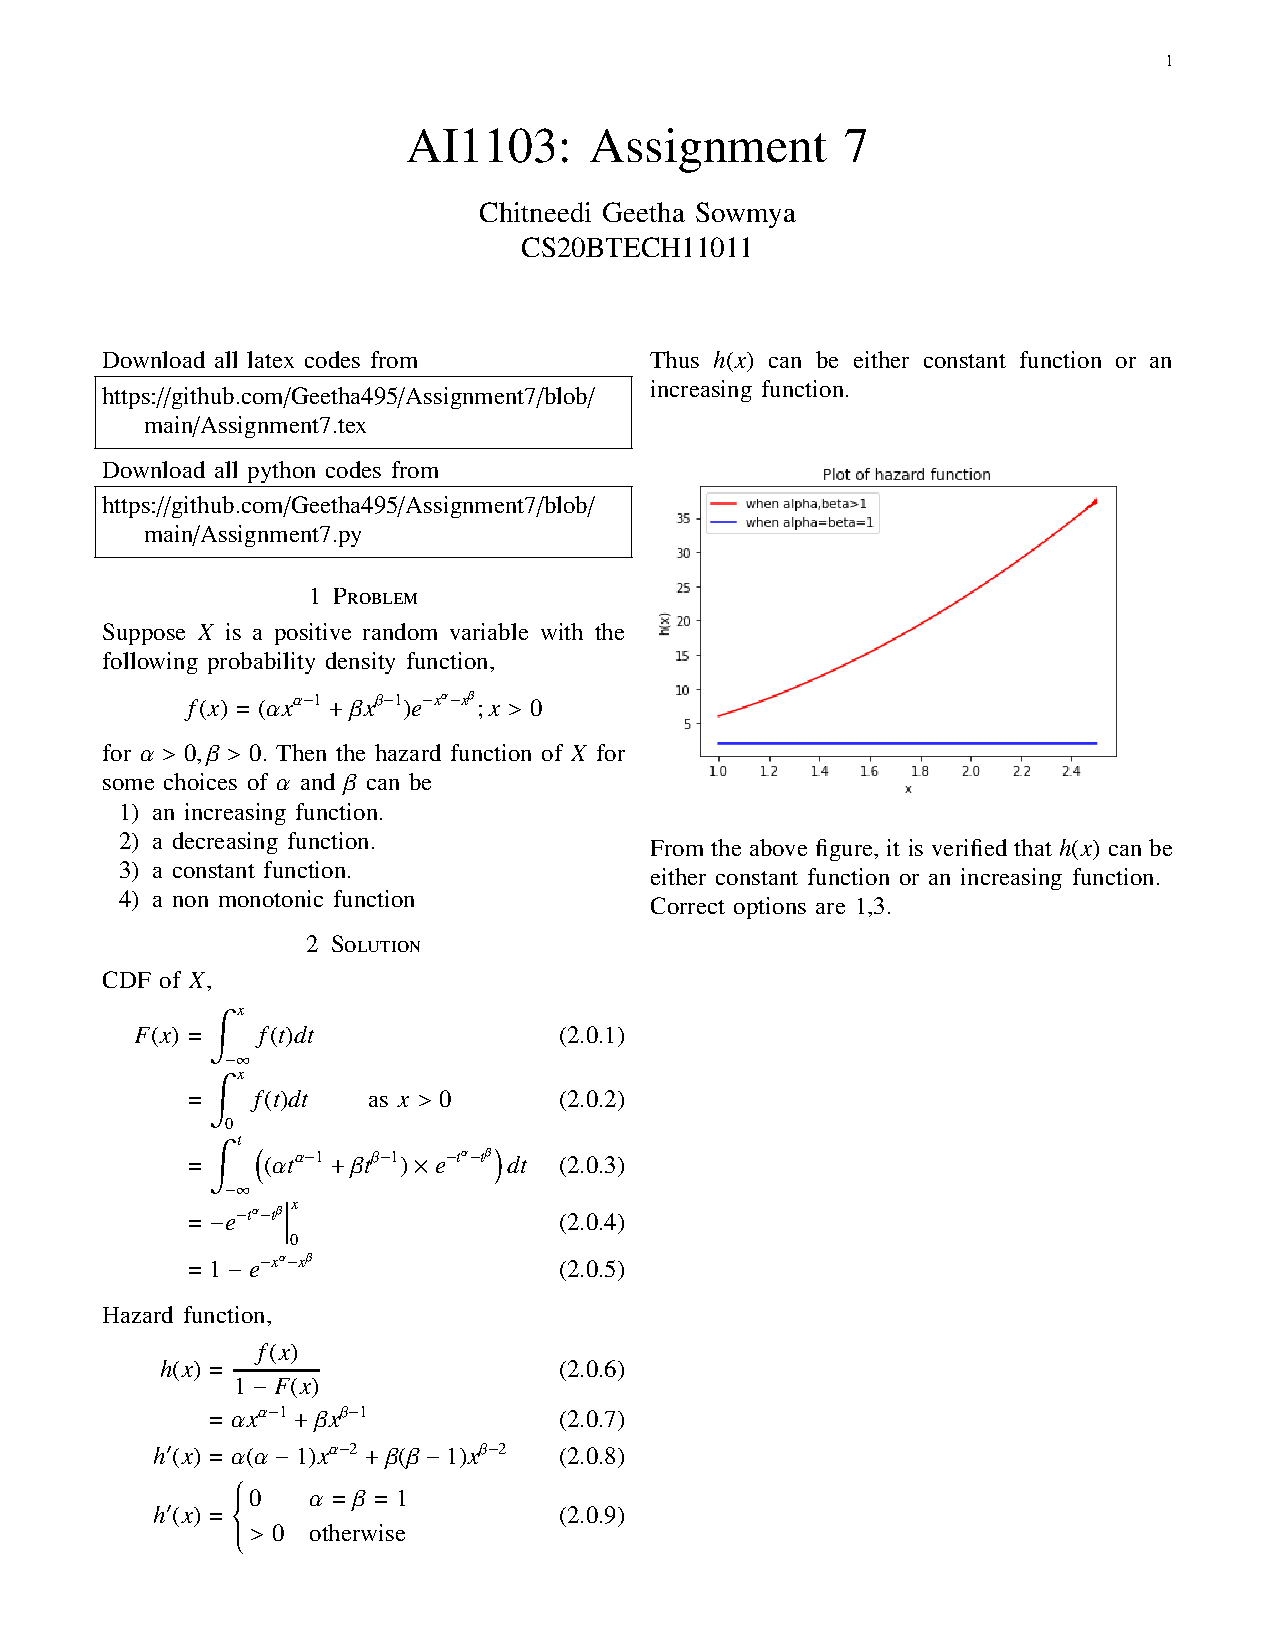
\includegraphics[width=\columnwidth]{Assignment7.png}
% \caption{pdf of $ Y=sign(X)$}
% \label{june/2012/112/pdf}
% \end{figure}
\begin{align}
   \implies \mu_y = 0 
\end{align}
and variance is
\begin{align}
    \sigma_y^2 &= (-1)^2\brak{\frac{1}{2}}+(1)^2\brak{\frac{1}{2}}\\
    &=1
\end{align}
\item Given
\begin{align}
    S_n&=\sum_{i=1}^{n} sign(X_i)\\
    S_n(\theta=0)&=\sum_{i=1}^{n} Y_i
\end{align}
From central limit theorem 
\begin{align}
    Z&=\lim_{n\to\infty}\sqrt{n}\brak{\frac{\frac{S_n}{n}-\mu_y}{\sigma_y}}\\
    &=\lim_{n\to\infty}\sqrt{n}\brak{\frac{S_n}{n}}\\
    &=\lim_{n\to\infty}\brak{\frac{S_n}{\sqrt{n}}}
    \label{june/2012/112/clt}
\end{align}
where Z is a standard normal variable N(0,1).
\begin{enumerate}
    \item Given
\begin{align}
    \alpha = P\cbrak{Z>z_\alpha}\label{june/2012/112/uff}
\end{align}
So from $\eqref{june/2012/112/clt}$ and $\eqref{june/2012/112/uff}$
\begin{align}
\lim_{n\to\infty}P\cbrak{\frac{S_n}{\sqrt{n}}>z_\alpha}&=
\alpha\\
\implies \lim_{n\to\infty}P\cbrak{S_n>\sqrt{n}z_\alpha}&=
\alpha
\end{align}
\end{enumerate}
\end{enumerate}
{$H_1:\theta >0$ is true}
\begin{enumerate}
    \item Given X is symmetric around $\theta>0$.Let us assume $\theta=\theta_0>0$.
    \begin{align}
        f_X(\theta_0-x)&=f_X(\theta_0+x)\\
        \int_{\theta_0}^{\infty} f_X(\theta_0-x)dx&=
        \int_{\theta_0}^{\infty} f_X(\theta_0+x)dx
        \label{june/2012/112/s}
    \end{align}
    \begin{enumerate}
        \item Solving LHS of $\eqref{june/2012/112/s}$.Changinng $(\theta_0-x) \rightarrow t$
        \begin{align}
           \int_{\theta_0}^{\infty} f_X(\theta_0-x)dx&=
           \int_{-\infty}^{0}f_X(t) dt\\
           &=\pr{X\leq0}\label{june/2012/112/temp}
        \end{align}
        \item Solving RHS of $\eqref{june/2012/112/s}$.Changing $(\theta_0+x) \rightarrow t$
        \begin{align}
           \int_{\theta_0}^{\infty} f_X(\theta_0+x)dx&=
           \int_{2\theta_0}^{\infty} f_X(t)dt\\
          &= \int_{0}^{\infty} f_X(t)dt-\int_{0}^{2\theta_0} f_X(t)dt\\
          &=\pr{X\geq0}-k\label{june/2012/112/u}
        \end{align}
        where
        \begin{align}
           k=\int_{0}^{2\theta_0} f_X(t)dt>0 
        \end{align}
    \end{enumerate}
    From $\eqref{june/2012/112/s}$,$\eqref{june/2012/112/t}$ and $\eqref{june/2012/112/u}$
    \begin{align}
        \pr{X\geq0}>\pr{X\leq0}
    \end{align}
    \item So
    \begin{align}
        \pr{Y=1}>\pr{Y=-1}
    \end{align}
    Therefore,if we perform the experiment and find the value of $\brak{\frac{S_n}{\sqrt{n}}}$,it is most likely to occur on the right side of the distribution of 
$\brak{\frac{S_n}{\sqrt{n}}}$.In $\eqref{june/2012/112/clt}$ it is shown that distrubution of the random variable $\brak{\frac{S_n}{\sqrt{n}}}$
 is $N(0,1)$ when n is very large.So
\begin{align}
    \lim_{n\to\infty}P\cbrak{\frac{S_n}{\sqrt{n}}>Z_\alpha}=1
\end{align}
\end{enumerate}
%


\end{enumerate}